\part{Vector products}
\frame{\partpage}

\begin{frame}{Dot and cross product}
	\pause $$a \cdot b = |a| |b| \cos \theta$$
	where $\theta$ is the \textbf{angle} between $a$ and $b$
	\vspace{2ex}
	\pause $$a \times b = (|a| |b| \sin \theta) n$$
	where $n$ is a unit vector \textbf{perpendicular} to both $a$ and $b$
	with direction given by the \textbf{right-hand rule}
\end{frame}

\begin{frame}{Uses}
	\begin{itemize}
		\pause\item Both dot and cross product are \textbf{quick to calculate}
		\pause\item Dot product can be used to find the \textbf{angle} between vectors
			\begin{itemize}
				\pause\item Actually the \textbf{cosine} of the angle
				\pause\item If $a \cdot b = 0$ (and $a,b$ are non-zero) then $\cos \theta = 0$, i.e.\ $\theta = 90^\circ$: $a$ and $b$ are \textbf{perpendicular}
				\pause\item If $a \cdot b = 1$ and $a,b$ are unit vectors then $\cos \theta = 1$, i.e.\ $\theta = 0^\circ$: $a$ and $b$ are \textbf{parallel}
			\end{itemize}
		\pause\item Cross product can be used to find a vector \textbf{perpendicular} to two others
	\end{itemize}
\end{frame}

\begin{frame}{Surface normals}
	\begin{columns}
		\pause
		\begin{column}{0.33\textwidth}
			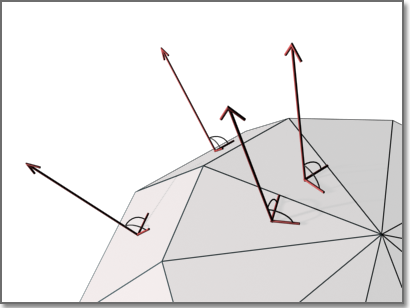
\includegraphics[width=\textwidth]{surface_normal}
		\end{column}
		\begin{column}{0.65\textwidth}
			\begin{itemize}
				\item The \textbf{normal} to a surface is a \textbf{unit vector} that is \textbf{perpendicular} to the surface
				\pause\item If we have two non-parallel vectors that are \textbf{tangent} to the surface, we can use the \textbf{cross product} to find the normal
			\end{itemize}
		\end{column}
	\end{columns}
	\pause
	\begin{columns}
		\begin{column}{0.33\textwidth}
			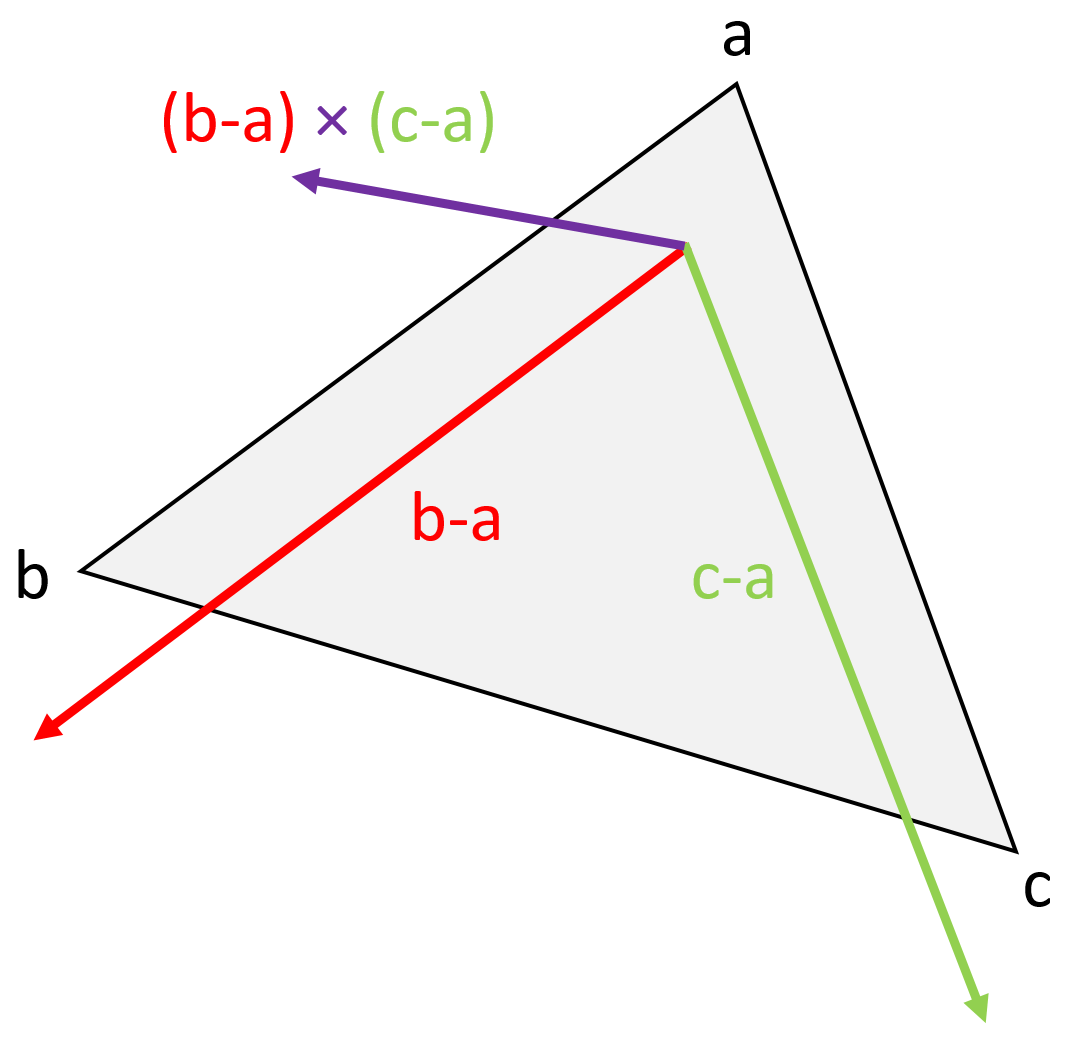
\includegraphics[width=\textwidth]{triangle_normal}
		\end{column}
		\begin{column}{0.65\textwidth}
			\begin{itemize}
				\item For a triangle with vertices $a, b, c$, two such vectors are $b-a$ and $c-a$
				\pause\item So the normal is
					$$ \frac{n}{|n|} \quad \text{where} \quad n = (b-a) \times (c-a) $$
			\end{itemize}
		\end{column}
	\end{columns}
\end{frame}
